\chapter{Experiments and Results}
\label{experiments_and_results}

\section{Investigating the Function Signature} % (fold)
\label{sec:investigating_function_sig}

% INVESTIGATION PURELY BASED ON NAME
\subsection{Comparing Baseline Models} % (fold)
\label{sub:comparing_baseline_models}


% We focused on the signature because of the important nature of this section of the code. 
% In langugages such as C++, the signature of function may be all that is presented to the user of a third-party library, when using that library. 
% Therefore being able to generate reasonable descriptions from signature items alone would already be of value. 
% This does not seem an unrealistic target, since good developer practice often involves giving insightful names to variables and functions\footnote{https://github.com/google/styleguide/blob/gh-pages/pyguide.md\#s3.16-naming}.



\subsubsection{Experiment Objective} % (fold)

As a baseline, we first wanted to investigate the informative power of simply the name of each argument with regards to different architectures of our model.
% As a baseline, we first wanted to investigate the informative power of simply the name of each argument with regards to different architectures of our model.
Since good developer practice often involves giving insightful names to variables\footnote{https://github.com/google/styleguide/blob/gh-pages/pyguide.md\#s3.16-naming}, we hypothesized that
 both our Rote Learner and Seq2Seq models should able to generate a plausible description using just the name of the argument.
We wanted to use this opportunity to investigate the relative performance of different features of the Seq2Seq model.

\subsubsection{Method \& Results} % (fold)

Since this experiment would only use the variable name to predict the descrption, we used the \textbf{Reduced Random-Split Dataset} listed in Table \ref{tab:final_datasets}.
This prevented inflation of BLEU scores due to exact matches being both in the train and validation set.
% TODO: As comparison, see how much BLEU score increases & decreases 

We ran our Rote Learner model as described in Section \ref{sec:general_procedure}. We then ran our on the basic Seq2Seq architectures in an ablation study: we started from a basic seq-to-seq, then adding attention, a bidirectional encoder and finally dropout.
These models were trained for a maximum of 150 epochs, in the manner as outline in section \ref{sec:general_procedure}, with our best model on validation set selected. 
The hyperparameters for these models are found in Appendix Table \ref{table:hyperparams_name_baseline}.
 % WHY 150

We report our corpus-level BLEU-4 scores in Table \ref{table:name_baseline}, and confirm our hypothesis that just argument name is a valuable indicator for generating descriptions. We note a strong BLEU-4 score from the Rote Learner of $9.03 \pm 0.32$ on validation and $10.60 \pm  0.30$ on test, which demonstrates the informativeness of simple n-character subsequences. 
This is surpassed by the bidirectional Seq2Seq with attention and dropout,  which achieves a BLEU-4 score of $12.68 $ and $12.72$ on validation and test set respectively.
In our ablation study we note the improvement that each new feature adds, noting that the pure Seq2Seq model underperforms the Rote Learner, scoring $8.97$ and $ 8.18 $ on the validation and test set. 

% ALL STOPPED at 150 EPOCHS. No improvement on best for 20 epochs, except original 146


\begin{table}[!ht]
\begin{center}
\begin{tabular}{ c | c | c }
    Model                             & BLEU (Validation)  & BLEU (Test)    \\
    \hline
    Rote Learner (x50)                & $ 9.03 \pm  0.32 $ & $ 10.60 \pm 0.27 $   \\
    \hline
    Seq to Seq                        & $ 8.97 $ & $ 8.18 $ \\
    + \textit{attention}              & $ 10.05 $ & $ 9.89 $  \\
    + \textit{bidirectional encoder}  & $ 11.76 $ & $ 12.34 $  \\
    + \textit{dropout}                & $ 12.68 $ & $ 12.72 $  \\
    \hline

    % Model                             & BLEU (Validation)  & BLEU (Test)    \\
    % \hline
    % Rote Learner (x50)                & $ 9.03242 \pm  0.31980 $ & $ 10.59658 \pm 0.26939 $   \\
    % \hline
    % Seq to Seq                        & $ 8.98624 $ & $ 8.17635 $ \\
    % + \textit{attention}              & $ 10.05134 $ & $ 9.88608 $  \\
    % + \textit{bidirectional encoder}  & $ 11.75615 $ & $ 12.34480 $  \\
    % + \textit{dropout}                & $ 12.67504 $ & $ 12.72236 $  \\
    % \hline
    % Seq to Seq                        & $ 4.60169 $ & $ 4.97880 $  \\
    % + \textit{attention}              & $ 4.81255 $ & $ 5.42022 $  \\
    % + \textit{bidirectional encoder}  & $ 3.00068 $ & $ 3.05952 $  \\
    % + \textit{dropout}                & $ 6.37864 $ & $ 6.33307 $  \\
    % \hline
\end{tabular}
\caption {Results of Experiment Comparing Baseline Models}
\label{table:name_baseline}
\end{center}
\end{table}



\subsubsection{Analysis} % (fold)
We were most surprised by the strength of Rote Learner on this dataset. Given there are no exact matches of (name, description) pairs in this dataset, we were curious to see where the performance had come from.
We examined the predictions of the Rote Learner on the validation set by taking their sentence-level BLEU-4 scores, and reading the predictions.
We found that although the vast majority evaluate to zero, a number of examples have a coincidental overlap in descriptions, resulting in a non negligible BLEU score. 
A number of examples also have the same name and almost identical descriptions, giving some predictions very high BLEU scores.
A random sample of these non-zero sentence-level BLEU translations are presented in Figure \ref{tab:rotelearner_nameonly}.


% This is largely the result of there are arguments in the corpus with very similar descriptions, which may vary by only a few words. 

% To investigate this we examined the predictions from the Rote Learner on the validation set. 
% We evaluated the sentence level BLEU score on these, and found that although the vast majority evaluate to zero, a number of examples have a coincidental overlap in descriptions, resulting in a non negligible BLEU score. 
% A random sample of these non-zero scored translations are presented in Figure \ref{tab:rotelearner_nameonly}.


With then examined the Seq2Seq model and ablation study. We were not surprised that the additions each improved the performance of the model in some way. The bidirectionality adds capacity to the model by increasing the size of the hidden vector, and prevents the model forgetting elements at the start of long sequences. The attention allows the model to condition each generated word on the encoder outputs, adding complexity to the model.
The dropout also adds a regularizing effect.
Each of these should improve the performance of the model.

% With regard to the Seq-to-Seq, it is not surprising these standard additions to the seq-to-seq architecture improve the model. 
% The addition of a bidirectional model adds capacity to the model by increasing the size of the hidden vector, and attention allows the model to condition sentence generation on the input, further adding complexity to the model.
% The dropout also adds a regularizing effect.

We were interested to note that the basic Seq2Seq narrowly underperforms the Rote Learner. 
It is possible that without the contextualising information from attention, the model struggles to learn from long description sequences. In contrast, the Rote Learner can regurgitate these immediately. 

Once the attention is added, and the capacity increased, the Seq2Seq's outperformance of the Rote Learner is explanatory.
The Seq2Seq synthesises similar (or even the same!) sequences of characters, with different descriptions, into a single description, which may fit better than randomly guessing from a bag of seen sequences. 

For instance, the most frequent argument, \mintinline[]{yaml}{name}, occurs in the train set 318 times with different descriptions. 
It also occurs 52 times in the validation set, again, with different descriptions. 
For each of these points the Rote Learner predicts a different description from the train set, due to its inherent randomness. On average it scores $0.00646 \pm 0.006$ in sentence BLEU. The Seq-to-Seq, by contrast, makes the \textit{same} prediction each time, and scores $0.4029$, almost two orders of magnitude better. Examining the predicted description of this argument confirms a sensible guess: \mintinline[]{yaml}{name} - \textit{``name of the variable to return."} 

In these cases the Seq2Seq model is interpolating in an overdetermined problem, and this highlights one of the advantages of neural networks in machine translation problems. 

\begin{table}
\begin{center}
\makebox[\linewidth][c]{
\begin{tabular}{l}
\hline\\

\textbf{A Random Sample of Sentence BLEU-4 Scores $>0$ from Rote Learner on Random Split }\\\\ 


\textbf{BLEU Score}: 0.364
\textbf{Confidence}: 100.0\%  \\
\textbf{Argument}: \mintinline[]{python}{e d g e _ m a t c h}\\
\textbf{Description}: a function that returns true if the edge attribute dictionary for \\
the pair of nodes ( u1 , v1 ) in g1 and ( u2 , v2 ) in g2 should be considered equal during\\
the isomorphism test . if edge\_match is not specified then edge attributes are not considered .\\
\textbf{Prediction}: a function that returns true if the edge attribute dictionaries for\\
the pair of nodes ( $<$UNK$>$ , $<$UNK$>$ ) in $<$UNK$>$ and ( u2 , $<$UNK$>$ ) in $<$UNK$>$\\
should be considered equal during matching .\\

\\
\textbf{B}: 0.075
\textbf{C}: 11.1\%  \\
\textbf{A}: \mintinline[]{python}{u s e _ l o c k i n g}\\
\textbf{D}: ` bool ` . if true use locks for update operation .\\
\textbf{P}: an optional ` bool ` . defaults to ` true ` . an optional bool . defaults to\\
true . if true , the assignment will be protected by a lock ; otherwise the behavior is\\
undefined , but may exhibit less contention .\\
\\
\textbf{B}: 0.558
\textbf{C}: 12.5\%  \\
\textbf{A}: \mintinline[]{python}{y _ t r u e}\\
\textbf{D}: ground truth ( correct ) target values .\\
\textbf{P}: ground truth ( correct ) labels .\\
\\
\hline
\\
\end{tabular}
}
\end{center}
\caption{A random sample of sentence level BLEU-4 scores that are non-zero on the validation set for a Rote Learner. We note that in the last example, the Rote Learner returns an almost identical description with 12.5\%, confidence, and in the first example returns a very similar description with 100\% confidence.}
\label{tab:rotelearner_nameonly}
\end{table}


% INVESTIGATION DIFFERENT TOKENIZATIONS
\subsection{Investigating Different Parts of the Signature} % (fold)
\label{sub:investigating_different_tokenizations}

\subsubsection{Experiment Objective} % (fold)

% We hypothesized that langugages such as C++, the signature of function may be all that is presented to the user of a third-party library\footnote{in the form of \mintinline[]{python}{.h} header file and binary}, when using that library. 
We noted that in many languages\footnote{such C++, C, C\#, which encourage the use of header file + binary, in library development} 
a developer may only have access to the function signature in trying to determine what a variable may be. Therefore quality naming is often important for all parts of the function signature.\footnote{https://google.github.io/styleguide/cppguide.html\#Names\_and\_Order\_of\_Includes}
Having established a naive baseline and the validity of our neural approaches, we decided to investigate how other function signature features could help generate our argument descriptions.
We hypothesised that the other names in the function signature could play an important role in contextualising an overdetermined or underdetermined variable name, further improving the performance of the Seq2Seq relative to the Rote Learner. 


\subsubsection{Method \& Results} % (fold)

We investigated how four different tokenizations of function signature data would affect translation behaviour for both our Rote Learner, and our strongest Seq2Seq. 
These tokenizations were:
\begin{tight_enumerate}
    \item just the argument name
    \item the argument name with the function name
    \item the argument name with co-argument names 
    \item the argument name with both function name and co-argument names
\end{tight_enumerate}

Once again we used the \textbf{Reduced Random-Split Dataset}, to prevent advantages due to duplicates, ran tokenization procedures outlined previously, and followed the general procedure outlined in Section \ref{sec:general_procedure}. For our Seq2Seq, we used the best arrangement from our first experiment, including a bidirectional encoder, attention and dropout. We ran these for 150 epochs, and selected the best, just as in Section \ref{sub:comparing_baseline_models}. The hyperparameters for our trainng are presented in Appendix Table \ref{table:hyperparams_different_tokenizations}.

We report our corpus level BLEU-4 results in Table \ref{table:tokenization}. 
We note that in all cases the Rote Learner's performance improved with added information, confirming that character overlap in the function signature can be an indicative feature in generating argument description.
In it's best case the Rote Learner improved over three points to $12.22 \pm 0.23$ on validation and $14.34 \pm 0.21$ on test, thanks to the addition of the function name. 

The Seq2Seq model on the other hand benefitted less than the Rote Learner, if at all. In both tokenizations using co-arguments, the model improved by approximately one point. However the tokenization of argument name and function name saw a performance reduction of about 1.5 points, across both validation and test.

Although this agreed with out hypothesis that there is value in extra naming of variables, the underperformance of the Seq2Seq model was surprising and is examined in detail in the analysis section.

\begin{table}[!ht]
\begin{center}
\begin{tabular}{ c | c | c }
    Model                               & BLEU (Validation)            & BLEU (Test)  \\
    \hline
    \hline
    Rote Learner                        &                  & \\    
     \textit{name only}                & $ 9.03  \pm  0.32 $ & $ 10.60 \pm 0.27 $  \\
     \textit{name + function name}     & $ 12.23 \pm  0.23 $ & $ 14.34 \pm 0.22 $  \\
     \textit{name + co-argument names}        & $ 12.06 \pm  0.16 $ & $ 14.22 \pm 0.16 $  \\
     \textit{name + function name + co-argument names}  & $ 11.36 \pm  0.14 $ & $ 13.51 \pm 0.13 $ \\
    \hline
    \hline
    Seq to Seq                          &                  & \\
     \textit{name only}                & $ 12.46441 $ & $ 12.72522 $  \\
     \textit{name + function name}     & $ 10.77699 $ & $ 11.24894 $ \\
     \textit{name + co-argument names}      & $ 13.69964 $ & $ 13.73890 $  \\
     \textit{name + function name + co-argument names} & $ 14.13267 $ & $ 13.63351 $ \\
    % Model                               & BLEU Validation            & BLEU Test  \\
    % \hline
    % \hline
    % Rote Learner                        &                  & \\    
    % - \textit{name only}                & $ 9.03242  \pm  0.31980 $ & $ 10.59658 \pm 0.26939 $  \\
    % - \textit{name + function name}     & $ 12.22728 \pm  0.23408 $ & $ 14.33850 \pm 0.21622 $  \\
    % - \textit{name + co-argument names}        & $ 12.06262 \pm  0.16356 $ & $ 14.21676 \pm 0.16067 $  \\
    % - \textit{name + function name + co-argument names}  & $ 11.35728 \pm  0.13663 $ & $ 13.50626 \pm 0.13192 $ \\
    % \hline
    % \hline
    % Seq to Seq                          &                  & \\
    % - \textit{name only}    !!            & $ 12.46441 $ & $ 12.72522 $  \\
    % - \textit{name + function name} !!    & $ 10.77699 $ & $ 11.24894 $ \\
    % - \textit{name + co-argument names}  !!    & $ 13.69964 $ & $ 13.73890 $  \\
    % - \textit{name + function name + co-argument names}   !! & $ 14.13267 $ & $ 13.63351 $ \\
    % \hdashline
    % Seq to Seq                          &                  & \\
    % - \textit{name only}                & $ 5.54103 $ & $ 5.43827 $  \\
    % - \textit{name + function name}     & $ 4.76165 $ & $ 4.40557 $  \\
    % - \textit{name + other args}        & $ 5.70546 $ & $ 6.04723 $  \\
    % - \textit{name + function name + other args}     & $ 6.26783 $ & $ 6.24153 $ \\
    
    \hline
\end{tabular}
\caption {Results of the experiments using different parts of the signature}
\label{table:tokenization}
\end{center}
\end{table}


\subsubsection{Analysis} % (fold)
\label{ssub:analysis}

In order to probe the Seq2Seq model, we first investigated the predictions qualitatively, reading the descriptions generated on the validation set. 
We found that many of the errors fell into either the categories of overfitting or nonsense. 
However, we also found descriptions where the model seemed plausible, with a good degree of fluency.
To illustrate this clearly, some typical examples of the model on the \textit{name + co-argument name} model are presented in Table \ref{table:typicalvarotherargs}. 


\begin{table}[ht!]
\begin{center}
\begin{tabular}{ l  }


\textbf{Overfitting}\\

\textbf{Input}: \mintinline[]{python}{e n c o d i n g _ t y p e <S1> s e l f <S2> d o c u m e}...\\
...\mintinline[]{python}{n t <S2> r e t r y <S2> t i m e o u t <S2> <END>}\\
\textbf{Description}: the encoding type used by the api to calculate offsets .\\
\textbf{Prediction}: the encoding type used by the api to calculate sentence offsets . \\
\\\hline\\

\textbf{Nonsense}\\

\textbf{I}: \mintinline[]{python}{i n p u t <S1> n a m e <S2> <END>}\\
\textbf{D}: a ` tensor ` of type ` complex64 ` . a complex64 tensor .\\
\textbf{P}: ` $<$UNK$>$ ` , ` $<$UNK$>$ ` . shape is ` [ ... , m , m ] ` . \\
\\\hline\\

\textbf{Plausible}\\

\textbf{I}: \mintinline[]{python}{i n p u t <S1> s t r u c t u r e <S2> m a s k <S2> o u t p}...\\
...\mintinline[]{python}{u t <S2> b o r d e r _ v a l u e <S2> o r i g i n <S2> <END>}\\
\textbf{D}: binary image to be propagated inside ` mask ` .\\
\textbf{P}: binary image where a element is provided and a structuring element .\\
\\\hline\\

\\

\end{tabular}
\caption{Three examples of typical errors in the character Seq-to-Seq model.
The first example is an example of overfitting where the whole predicted sentence is found in the training set.  The second example is nonsensical, with lots of $<$UNK$>$ tokens.  In the final case, the predicted sentence is original and shows features of the desired sentence. 
}
%multiple sequences such as these are found in the dataset, each with a different discription. Without looking at code, or function name (in this case) it is impossible to disambiguate and the model fails to make sense }
\label{table:typicalvarotherargs}
\end{center}
\end{table}

We then visualized a number of attentions of the translations on the validation set, to investigate what the model was focusing on in these cases.
We found that, rather than being dispersed across multiple tokens that might indicate useful phrases in the model, the attention focused overwhelmingly on the final tokens in the RNN in the vast majority of cases.
The attentions of the `plausible' and `nonsense' examples from  Table \ref{table:typicalvarotherargs} are visible in Figure ~\ref{fig:otherarg_attn}, demonstrating this.

\begin{figure}[ht!]
\begin{center}
    % \includegraphics[width=0.7\linewidth]{images/otherargs_example.png}
    \includegraphics[width=0.9\linewidth]{ImagesCodeRelated/attn1pretty.png}
    \includegraphics[width=0.5\linewidth]{ImagesCodeRelated/attn2pretty.png}
    \caption{An example of some the attentions of from the Name + Other Arguments tokenization on a Seq-to-Seq model, on the Reduced Random-Split Dataset. The top a picture is a typical example from the dataset, where all attention is on the last two tokens which (in this tokenization) never change.  The bottom is a less typical example that occurs when the character sequence is very overdetermined.}
    \label{fig:otherarg_attn}
\end{center}
\end{figure}

This implies the model is not learning to apply parts of the sequence to parts of the translation, in the alignment fashion demonstrated by \citet{bahdanau_neural_2014}. Instead it appears to be using all the encoded input information to create (almost) the same single vector to contextualise on at each step.
% This implies the model is using all the extra information to encode a single vector to contextualise on, rather than learning to apply parts of the sequence to parts of translation, in the alignment fashion demonstrated by Bahdanau\cite{bahdanau_neural_2014}.
This single contextual vector can contain all the input sequence information because, in an RNN, the encoder outputs at step $N$ can contain information from the previous $N-1$ tokens. This in principle allows the model to condition word generation on the all the information up to the final `attended' encoded token. 

Although this behaviour was expected for short sequences like variable names, we expected longer sequences (of up to 120 tokens) to be harder to compress, and suspected overcapacity of the LSTM might allow this learning strategy to take place. 
With less capacity, perhaps the final output of the RNN would not be as informative. It would then be forced to rely on outputs at different points of the sequence - perhaps indicating where the argument name ends, or where an informative sequence of characters lies.
However, repeating the experiment with an LSTM encoder with a much smaller hidden state (75 dimensions), resulted in the exactly the same pattern of attention, though with a much reduced BLEU score.

We also repeated the experiment on the larger \textbf{Full Random-Split} dataset. In this case the input argument name would be certainly be the most important feature, due to the repetition of points with the same name and description but different signatures. 
In this case we saw the attention shift from the last token(s) to the separator token just after the variable name. This indicated that the model was learning where the most informative section of the data was, but was still only attending to a single point.
 % We hypothesized it was using the same strategy of using the constant attention vector to guide the type of description generated at each step.
This raised the worrying possibility that the network was not even using the encoding intermediate vector, in its decoding in this case.

To disprove this possibility, we needed to check that the rest of the sequence was still being used in decoding. Therefore we took the test sequence and truncated at different points. We found that model did still take into account the rest of the sequence after the separator token, since it generated different translations, but that these all varied along a the same theme of the variable name. This is visible in Figure \ref{fig:otherarg_attn_full_dataset}. This supported our suggestion that the attention vector was being treated as a contextualising vector in decoding, strongly guiding the type of description generated.


\begin{table}
\centering
\makebox[\linewidth][c]{
% \makebox
\begin{tabular}{rcl}
    \includegraphics[width=0.39\linewidth]{images/trimmed1.png} &
    \includegraphics[width=0.39\linewidth]{images/trimmed2.png}&
    \includegraphics[width=0.39\linewidth]{images/trimmed3.png}\\
    % \includegraphics[width=0.7\linewidth]{images/different_translations_dupsXotherargs_3230minib_white.png}
\end{tabular}
}
    \caption{The attentions from the \textit{name + co-arguments} tokenization on a Seq-to-Seq model trained on the Full Random-Split Dataset. In this dataset, the duplicates of (name, description) pairs make the name the most important feature, hence the attention at the separator token. However the rest of the sequence is still being used by the decoder, as the clipped input sequences still generate different descriptions.  
    % Here is shows that, on the Full Random-Split Dataset, the most important feature is variable name, and the model attends solely to that, but that the hidden state of the LSTM still takes into account characters after the variable input
     }
    \label{fig:otherarg_attn_full_dataset}
\end{table}

One conclusion to be drawn from this overall investigation is that the attention has not distributed well over characters, failing to pick out individual features. Instead, with these tokenizations, the neural network seems to treat the signature strings like much longer single names. 
This has led to overfitting in many cases, as the new `names' are more likely to be unique. In cases such as argument name + function name this seems to lead the network down the wrong path. It also suggests why the Seq2Seq model might not be outperforming  the Rote Learner in our corpus-level BLEU score. 

However we can also conclude from this experiment that the function signature is capable of providing information to generate documentation - as visibile from the Rote Learner - and that neural methods seem a good way to do this.
 % to decode variable descriptions (as seen from our Rote Learner), and that neural approaches can provide a way of doing this.
Unlike our Rote Learner, our Seq2Seq model is capable of generating completely new descriptions, often with good fluency and has numerous examples of doing so. This seems to work best when the Seq2Seq is assimilating information from different training points, instead of overfitting to one. 
% However, because of the  but this seems more difficult to do when so much identifying information is given without information on redundancy. 
To give an example, Table \ref{table:example_plausible_training} shows the `plausible' example given above, with all the different training instances that start in the same way - with \mintinline[]{yaml}{input<S1>structure}. 
Here one can see an original sentence, yet with certain features assimilated from the training, such as the use of \textit{``binary image"}. We note in this example a room for improvement. The potentially helpful input sequence \mintinline[]{yaml}{<S2>mask<S2>} appears to have been ignored by the Seq2Seq, despite appearing relevant to the description. 
Getting the model to pay attention to these points is the key to our recommendations for improving this type of model.

\subsubsection{Further Work}

We believe that they key to improving the model is encouraging the model to interrogate the different features of the function signature, whether these be substrings or tokens indicating substring type.
As a result we recommend two key areas of investigation as further work for this model: modifications to the attention mechanism and improvements to the tokenization. 

% From both these conclusions, we suggest further work should be done
% This indicates that perhaps the training data is not sufficient, or sufficiently well tokenized, or the attention too focused for the Seq2Seq to pickup that this section might be important.

% To counter this behaviour in future, more work could be done by investigating variations to the attention or  tokenization.
Our first suggestion of future work, is that modifications to the attention should be investigated to help it focus on multiple character outputs. 
One approach could be to replace the peaky softmax with a broader distribution in order to force the model to consider different sections of the data.
This could easily be done just be adding a parameter, $\alpha$ to control the entropy of the softmax equation, perhaps varying during during training:
\begin{align}
softermax(\mathbf{x_i}, \alpha) = \dfrac{e^{{\alpha}x_i}}{\sum_ie^{{\alpha}x_i}}
\end{align}
A better proposal, however, is to implement a structured attention, which is designed to encourage a sparse focus across contiguous segments (\textit{fusedmax}) or non-contiguous segments (\textit{oscarmax}) of the encoded sequence. \citep{niculae_regularized_2017}
This technique has previously been used to improve performance and interpretability in machine translation tasks 
\citep{niculae_regularized_2017}.
Another approach, would be to regularise the network by simply penalising it for being too confident in its attention, as has proven to be effective by \citet{pereyra_regularizing_2017}.

A second suggestion of further work is much simpler, involving our tokenization. Since we always tokenized in the same order (argument name, function, coargument) we missed an opportunity for data augmentation, that might help the network pay more attention to the different names in the signature. By adding duplicates with shuffled orders, and maybe even synonyms in descriptions, the model may learn a more generalisable descriptions.


\begin{table}
\begin{center}
\makebox[\linewidth][c]{
\begin{tabular}{l}

\hline
\textbf{Validation Example}\\

\textbf{I}: \mintinline[]{python}{i n p u t <S1> s t r u c t u r e <S2> m a s k <S2> o u t p}...\\
...\mintinline[]{python}{u t <S2> b o r d e r _ v a l u e <S2> o r i g i n <S2>}\\
\textbf{D}: binary image to be propagated inside ` mask ` .\\
\textbf{P}: binary image where a element is provided and a structuring element . $<$END$>$\\
\\\hline\\

\textbf{Training Examples} starting \mintinline[]{yaml}{i n p u t <S1> s t r u c t u r e}\\
\textbf{I}: \mintinline[]{yaml}{i n p u t <S1> s t r u c t u r e 1 <S2> s t r u c t u r}...\\
...\mintinline[]{yaml}{e 2 <S2> o u t p u t <S2> o r i g i n 1 <S2> o r i g i n 2 <S2> <END>}\\
\textbf{D}: binary image where a pattern is to be detected .\\
\\
\textbf{I}: \mintinline[]{yaml}{i n p u t <S1> s t r u c t u r e <S2> i t e r a t i o n s <S2> o u t }...\\
...\mintinline[]{yaml}{p u t <S2> o r i g i n <S2> m a s k <S2> b o r d e r _ v a l u e }\\
...\mintinline[]{yaml}{<S2> b r u t e _ f o r c e <S2> <END>}\\
\textbf{D}: binary array\_like to be closed . non-zero ( true ) elements form the subset to be closed .\\
\\
\textbf{I}: \mintinline[]{yaml}{i n p u t <S1> s t r u c t u r e <S2> o u t p u t <S2> o r}...\\
...\mintinline[]{yaml}{i g i n <S2> <END>}\\
\textbf{D}: n-dimensional binary array with holes to be filled\\
\\
\textbf{I}: \mintinline[]{yaml}{i n p u t <S1> s t r u c t u r e <S2> o u t p u t <S2> <END>}\\
\textbf{D}: an array-like object to be labeled . any non-zero values in ` input ` are counted as features...\\
...and zero values are considered the background .\\
\\
\textbf{I}: \mintinline[]{yaml}{i n p u t <S1> s t r u c t u r e <S2> i t e r a t i o n s <S2> m a s k }...\\
...\mintinline[]{yaml}{<S2> o u t p u t <S2> b o r d e r _ v a l u e <S2> o r i g i n <S2>}\\
...\mintinline[]{yaml}{b r u t e _ f o r c e <S2> <END>}\\
\textbf{D}: binary image to be eroded . non-zero ( true ) elements form the subset to be eroded .\\
\\
\textbf{I}: \mintinline[]{yaml}{i n p u t <S1> s t r u c t u r e <S2> i t e r a t i o n s <S2> m a s k}...\\
...\mintinline[]{yaml}{<S2> o u t p u t <S2> b o r d e r _ v a l u e <S2> o r i g i n <S2>}\\
...\mintinline[]{yaml}{b r u t e _ f o r c e <S2> <END>}\\
\textbf{D}: binary array\_like to be dilated . non-zero ( true ) elements form the subset to be dilated .\\
\\



\end{tabular}
}
\caption{A validation example and all of training points that start with the same sequence of characters: \mintinline[]{yaml}{i n p u t <S1> s t r u c t u r e}. These demonstrate that model is, to some degree, assimilating the information from its training data, in these very long sequences. }
\label{table:example_plausible_training}
\end{center}
\end{table}

%%% EXTRA PLOTS: Avergae attention over words
%%%.             Attention/Results of words shuffled



% What is the problem? Attention softmax is narrow and doesnt distribute well over characters, since there isn't really a one to one alignment. Instead what we see is the same behaviour as a much longer function name, where it works best when interpolating data. then give the plausibility

% Future work: Attention softmax is too narrow. Try a higher entropy distribution for character model
% Try a learning schedule
% Rotate the order of words, (done)
% Also more data.


% \begin{enumerate}
%     % \item we expected words to help choose bits in overdetermined cases. attention distributed across multiple words
%     % \item however we get attention focused on last word.
%     % \item The rnn final state acts as a good contextual vector for generation, we get good performance improvements on decoding
%     % \item The sort bonus is explained, but no change with longer.
%     \item It is possible the attention is being pathological. It's such a good strategy, that it stays there, and stops looking elsewhere, the weight decays to zero
%     % \item To investigate we ran with low lstm, -> no change in behaviour (LSTM 75), still tries to encode
%     \item We then tried to investigate if the rest of the data is being used (use the full dataset, and found that)
%     \item in cases with still degeneracy, attention is confused it panics (see bluring at end - can only explore nearest by states)
%     \item Check out Rote learner vs LSTM for "name" again. is it interpolating, or being a bad lstm (fitting bits of it, that dont transfer.)
%     \item We also take a closer look at the failures and notice a specific pattern. note tha in some cases the model works well, and. Basically hypothesise the size of the data with lack of indentifyin ginformation leads to overfitting, rather than just variable name which works.
% \end{enumerate}


\section{Investigating the Variable Path Contexts} % (fold)
\label{sec:investigating_the_computer_channel}

\subsection{Comparing Code2Vec Decoder to Baselines} % (fold)
\label{sub:comparing_code2vec_to_baselines}


\subsubsection{Experiment Objective} % (fold)

In our first examinations of the AST data, we aim to validate our initial hypothesis that by using just parts of the code, in the form of VPCs, we could generate reasonable argument descriptions.
In particular we wished to assess what possible tokenizations of code paths could prove most effective in doing this, so as to build as strong a Rote Learner model as possible. We could then fully compare this as a strong benchmark against our Code2Vec Decoder model.

\subsubsection{Method \& Results} % (fold)

For this experiment we used the \textbf{Full Random-Split Dataset}, to make the most of the different code paths associated with each argument.
We followed the tokenization procedure outlined in Section \ref{sub:code_tokenization}, using vocabulary size of 15000 for both path and terminal nodes. We then clipped the maximum number of paths per argument to 5000, due to memory constraints. 

We then ran our Rote Learner with our standard general procedure, using the four different VPC-only matching criteria, summarised earlier in Table \ref{tab:matching_summary}. These chose a description from a set of training samples in different ways: each either matched full VPCs or VPC subpaths; and each either chose from points proportional to their matches, or simply by taking the most matched points.
We ran these different methods to investigate what features might be most indicative for our learner that memorized features, and to find our whether any such features were informative in the first place.
%     \begin{tight_itemize}
%         \item  - combining samples with largest subpath overlap for each VPC in test, and chosing from that list. (\textbf{Sub Path Proportional})
%         \item combining samples with largest subpath overlap for each VPC in test, and chosing from the most frequent training point(s) in that list. (\textbf{Sub Path Max})
%         \item combining samples with full overlap for each VPC in test, and chosing from that list (\textbf{Full Path Proportional})
%         \item combining samples with full overlap for each VPC in test, and chosing from the most frequent training point(s) in that list. (\textbf{Full Path Max})
%     \end{tight_itemize}
% We ran these different matching criteria to investigate 

We also ran the Code2Vec Decoder with the same tokenizations and for a maximum of 100 epochs, since we saw little improvement after this point.
As usual we selected our model that performed best on our validation set.
The hyperparameters for this model are found in Table \ref{table:hyperparams_code2vec}.

We report our corpus-level BLEU-4 results in Table \ref{table:name_code2vec_solo}. We note that the Rote Learner performed best using the Max Context criterion, which matched points that fully overlapped the most with the VPCs of test. This achieved a reasonable BLEU score of $ 11.82 \pm  0.16 $ and  $ 12.61 \pm 0.12 $ on validation and test,. However, we noted that the Code2Vec Decoder significantly outperformed this, achieving a BLEU score of $ 18.94 $ and $ 18.13 $ on validation and test respectively.

% From the Rote Learning perspective, the next best criterion was the Sub Path Max, which achieved a corpus level BLEU score of $ 6.93 \pm  0.34 $ and $ 7.09 \pm 0.22 $ on validation and test respectively.  
% The two remaining Proportional criteria performed worst, each about 6 bleu points worse than their counterparts

These results first confirmed the informative power of VPCs, and suggested that full VPC overlap be an informative feature in describing arguments. It also confirmed the strength of our neural approach to modelling full, and showed great promise for the Code2Vec Decoder as a model.

% subsection comparing_code2vec_to_baselines (end)

\begin{table}[ht!]
\begin{center}
\begin{tabular}{ c | c | c  }
    Model                             & BLEU (Validation)  & BLEU (Test)      \\
    \hline
    Rote Learner                  &  &  \\
    \textit{Subpath Proportional}              & $ 0.71 \pm  0.13 $ & $ 0.74 \pm 0.07 $   \\
    \textit{Subpath Max}                       & $ 6.93 \pm  0.34 $ & $ 7.09 \pm 0.22 $  \\
    \textit{Full Path Proportional}            & $ 4.94 \pm  0.28 $ & $ 5.11 \pm 0.18 $  \\
    \textit{Full Path Max}                     & $ 11.82 \pm  0.16 $ & $ 12.61 \pm 0.12 $  \\
    \hline
    Code2Vec Decoder                             & $ 18.94 $ & $ 18.13 $  \\
    % \hdashline
    % Code2Vec                          & $ 12.64199 $ & $ 12.80257 $  \\
    \hline 
    % Model                             & BLEU Validaion  & BLEU (Test)      \\
    % \hline
    % Rote Learner (codeonly)           &  & & \\
    % - \textit{softest}                     & $ 0.70702 \pm  0.13979 $ & $ 0.73623 \pm 0.07094 $   \\
    % - \textit{soft}                        & $ 6.93465 \pm  0.33987 $ & $ 7.09349 \pm 0.21836 $  \\
    % - \textit{hard}                        & $ 4.94109 \pm  0.28153 $ & $ 5.11432 \pm 0.18345 $  \\
    % - \textit{hardest}                     & $ 11.82453 \pm  0.15695 $ & $ 12.61319 \pm 0.12093 $  \\
    % \hline
    % Code2Vec   !!                            & $ 18.93630 $ & $ 18.12909 $  \\
    % % \hdashline
    % % Code2Vec                          & $ 12.64199 $ & $ 12.80257 $ & \\
    % \hline
\end{tabular}
\caption {Results for Code2Vec Decoder and a series of code only Rote Learners on the Full Random Split Dataset}
\label{table:name_code2vec_solo}
\end{center}
\end{table}

\subsubsection{Analysis} % (fold)
\label{ssub:analysis}
Noting the superior performance of the Code2Vec Decoder model, we first examined the model qualitatively. We sampled points from the validation set, printed their source code and VPCs, and visualizied their attentions as they passed through the model.
We observed that although sometimes the model's attention fit overwhelming to a single path, more often than not the model distributed its attention over 4 or 5 paths, even if there were thousands to choose from.

\begin{listing}[h!] 
\begin{center}

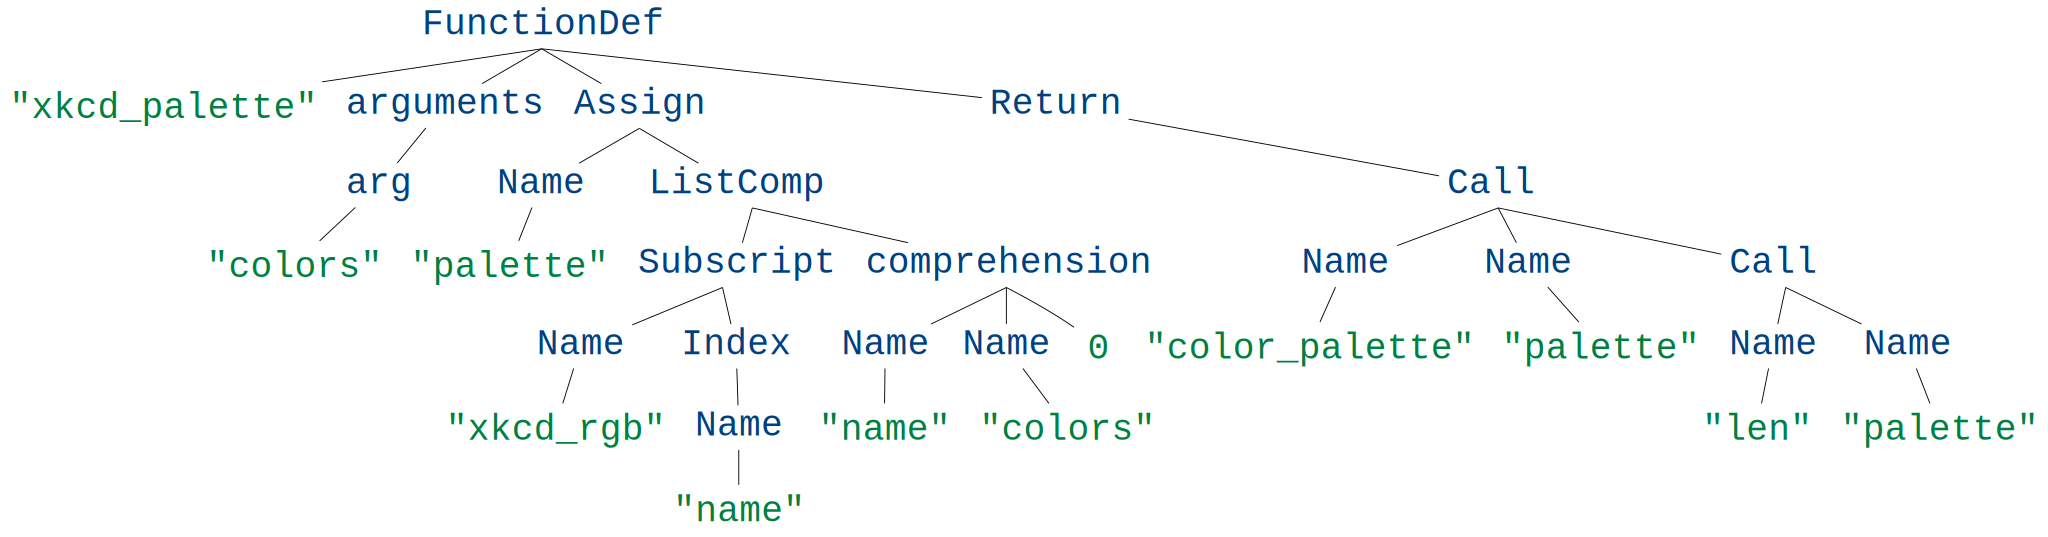
\includegraphics[width=\linewidth]{ImagesCodeRelated/xkcd_palette_strip.png}
\begin{minted}[]{python}
def xkcd_palette(colors):
    palette = [xkcd_rgb[name] for name in colors]
    return color_palette(palette, len(palette))

\end{minted}
\begin{tabular}{l}
\hline
\textbf{Argument Name}: \mintinline[]{python}{colors}\\
\textbf{Description}: list of keys in the `` seaborn.xkcd\_rgb `` dictionary .\\
\textbf{Prediction}: a list of data to read . if none , all other the first will be returned .\\
\end{tabular}
\end{center}
\caption{A pruned AST from which VPCs were extracted, and its source representation below. Below that the predictions that the Code2Vec Decoder made on the snippet of source. The predicted description correctly identifies a list.}
\label{fig:single_examples_code}
\end{listing}


\begin{listing}[ht!]
\begin{center}

\includegraphics[width=0.9\linewidth]{ImagesCodeRelated/pretty_attention_XKCD.png}
        % how to set font size here to 10 px ?  
\begingroup
    \fontsize{10pt}{12pt}\selectfont
\begin{tabular}{c l}
    & \textbf{Paths} \\
    \\
    \textbf{Path A} & Name $\uparrow$ comprehension $\uparrow$ ListComp $\downarrow$ comprehension : \mintinline[]{yaml}{<UNK>} \\
    \textbf{Path B} & Name $\uparrow$ comprehension $\uparrow$ ListComp $\uparrow$ Assign $\downarrow$ Name : \mintinline[]{yaml}{palette} \\
    \textbf{Path C} & Name $\uparrow$ comprehension $\downarrow$ Name : \mintinline[]{yaml}{name} \\
    \textbf{Path D} & $<$UNK$>$ : \mintinline[]{yaml}{palette} \\
    \textbf{Path E} & $<$UNK$>$ : \mintinline[]{yaml}{palette} \\
    \textbf{Path F} & $<$UNK$>$ : \mintinline[]{yaml}{name} \\
    \textbf{Path G} & $<$UNK$>$ : \mintinline[]{yaml}{len} \\
    \textbf{Path H} & $<$UNK$>$ : \mintinline[]{yaml}{color_palette} \\
    \textbf{Path I} & $<$UNK$>$ : \mintinline[]{yaml}{<UNK>} \\
\end{tabular}
\endgroup

% \caption{Example Attention Scores}
% \end{table}

\end{center}
\caption{The attentions scores for the VPCs corresponding to code in Listing \ref{fig:single_examples_code}, for each of our Code2Vec models. It is interesting that Path B implies that our argument \mintline[]{python}{colors} is involved in a list comprehension and is highly weighted by most models.   }
\label{fig:single_examples}
\end{listing}




An illustrative example of such analysis is presented in Listings  \ref{fig:single_examples_code} and \ref{fig:single_examples}. 
Listing  \ref{fig:single_examples_code} shows the pruned AST, source code, and the models predictions, while Listing \ref{fig:single_examples} shows the attented VPCs, and their relative attention scores.
From this example it is interesting to note that the model has chosen two paths that indicate list comprehensions feature in the variable, and it has inferred that a list should feature in the description from the code alone.



\begin{figure}[h]
\begin{center}
\includegraphics[width=0.8\linewidth]{ImagesCodeRelated/code2vec_entropies.png}
\end{center}
\caption{The distribution of entropies of the attentions of the Code2Vec Decoder model across the validation set (\textit{red}). For comparison, distributions of entropies of corresponding uniform categorical attentions is also presented (\textit{blue}). This demonstrates that the model choses a small number of paths to attend to, even though the spread of possible paths may be great.}
\label{fig:entropy_code2vec}
\end{figure}


Having noted that the model seemed to be performing as expected on a qualitative level, we continued to investigate the model more quantitatively. 
Figure \ref{fig:entropy_code2vec} shows the distribution of the entropies of the attention in the Code2Vec model, for each point in the validation set. 
Presented alongside is the distribution of entropies that would have occured if every data point in the validation set had attained a uniform, categorical distribution as attention over its VPC context vectors.
The shift to a lower entropy clearly verifies that the Code2Vec's attention focuses on only a fraction of the paths, and, in some few cases (where the entropy is effectively 0) decides resolutely on single points.

We also investigated the sentence-level BLEU-4 scores across the validation set. This metric is prone to low scores (since 4-gram precision of 0 immediately nullifies the score), but gave us a good sense for where the performance improvements come from in the Code2Vec Decoder Model.
With this metric we noted both a significant increase in the Code2Vec Decoder's 1.0 scoring sentences (about 12\%), and also a similar increase in model's low scoring sentences.
This indicates both an improvement that may be down to some form of overfitting (the model is able to find arguments that are very similar, and have similar code paths), but also an improvement due to generating just a few of the correct words, as in the example presented above. A graph presenting the distribution of scores in presented in Figure \ref{fig:sentence_bleu}.



% more points now scored a perfect 1.0 score (approximately 12\% more), and significantly more points now In particular this demonstrated that significant number of points now scoreed over  200 more
% % Figure \ref{fig:sentence_bleu} shows the counts of sentence-level BLEU-4 score of each sentence in the validation set.
% % Although this sentence-level BLEU-4 is prone to low scores on individual sentences, since BLEU-4 evaluates to 0 if no 4-gram is present, we can use it to get a sense for where the performance improvements come from in the Code2Vec Decoder Model.
% From this graph it is one can see both a significant increase in the models 1.0 scoring sentences, and also a modest increase in low scoring sentences. 
% This indicates both an improvement that may be down to some form of overfitting (the model is able to find arguments that are very similar, and have similar code paths), but also an improvement due to generating just a few of the correct words, as in the example presented above. 



% \begin{enumerate}
%     \item With the code lstm we see some of the behaviour we like, but also, only overfitting. There is no sequence so in some cases, a path or a single variable can be informative, but it performs well.
%     \item See a single example and distribution of attention.
%     \item CLearly there are a lot of spikes compared to uniform. More masking the more spiking, though this is partly due to best bleu. Compare at cross entropy time?
%     \item Then look at, bleu per sentence, maybe av bleu per sentence per attn entropy.
%     \item Big COMPARE vs ROTE LEARNER - can we conclude this is worth more researcg?
%     \item Cna show how choices change w model for given example??

%     \item C2VEnc: does combining add anythin? More capacity, check weights.
% \end{enumerate}

% \begin{table}


% subsubsection analysis (end)

\subsection{Masking Identifiers in Code2Vec Decoder} % (fold)
\label{sub:comparing_code2vec_altered}

\subsubsection{Experiment Objective} % (fold)

The Code2Vec Decoder model uses a vocabulary of terminal nodes strings in its VPCs. 
% A VPC consists of a path $p$ and terminal node $n$ string. 
These terminal nodes strings are almost always object names, which could belong to local variables, built-in functions or even out-of-scope objects. 
We investigated masking these terminal node names by renaming them, to test the robustness of our model to trivial changes in  code structure. 
We investigated two scenarios: first where the co-arguments are renamed; and second where all the names (including built-in methods) are renamed.


% The Code2Vec Decoder model uses a vocabulary of terminal nodes strings to generate code paths. 
% Due to the python abstract syntax tree, these are almost always names, which could be either those of internal variables, built-in functions or even out-of-scope objects. 
% Therefore, in principle, the model could learn which variable names are used within certain functions, and make it prediction from these.
% We investigated masking these terminal node names, to be able to conclude that the path structure of AST was providing a valuable signal to the Code2Vec Decoder, beyond the ideosyncracies of variable and method naming.

\subsubsection{Method \& Results} % (fold)

We used the same dataset and tokenization procedure as described in Section \ref{sub:comparing_code2vec_to_baselines} to prepare the tokenized code paths as before.
Then we prepared two different masking procedures, to hide the terminal node from the models.

In the first masking, we masked the only the coarguments names in the VPCs.
We did this by creating new terminal node identifiers, for `first coargument', `second coargument', and so forth, and replacing the the relevant identifiers in all the VPCs.
This meant that the model could still recognise when two code paths belong to the same terminal node, but could not use names to link the coargument to any previously-seen variable.

In our second masking, we repeated this procedure, but provided new terminal nodes for every object in the function: `first object', `second object' and so on.
This meant that very indicative global variables were masked, but also any built-in method.
The model only had access to enough information to be able to distinguish terminal nodes within a function, it could not generalise to their use between functions.

As before, this model was trained for 100 epochs, with the hyperparameters visible in Table \ref{table:hyperparams_masking}.

We present the results in Table \ref{table:code_2_vec_masked}, noting that Coargument Masking only resulted in a slight performance drop, of one to two BLEU points, from the unmasked variables, while the Full Masking resulted in a significant drop of six BLEU points, but still surpassed the best Rote Learner baseline. 
We note this as a significant result, demonstrating the robustness of our Code2Vec Decoder, in being able to generate reasonable descriptions, even with every single object in a function renamed.



\begin{table}[ht!]
\begin{center}
\begin{tabular}{ c | c | c }
    Model                             & BLEU (Validation)  & BLEU (Test)    \\
    \hline
    Rote Learner (best performer)          & $ 11.82 \pm  0.16 $ & $ 12.61 \pm 0.12 $ \\
    \hline
    Code2Vec  Decoder                             &  &  \\
    \textit{No Masking}                               & $ 18.94 $ & $ 18.13$ \\
    \textit{Coargument Masking}              & $ 17.02 $ & $ 16.94 $ \\                  
    \textit{Full Masking}                & $ 13.28 $ & $ 13.07 $ \\
    % Rote Learner (best performer)          & $ 11.82453 \pm  0.15695 $ & $ 12.61319 \pm 0.12093 $ \\
    % \hline
    % Code2Vec                               & $ 18.93630 $ & $ 18.12909 $ \\
    % Code2Vec  (Coargument Masking)              & $ 17.01868 $ & $ 16.93701 $ \\                  
    % Code2Vec  (Full Masking)                & $ 13.27677 $ & $ 13.07374 $ \\
    \hline
\end{tabular}
\caption {Results of investigating the Code2Vec Decoder with masked terminal nodes.}
\label{table:code_2_vec_masked}
\end{center}
\end{table}


\begin{figure}
\begin{center}
\includegraphics[width=0.8\linewidth]{ImagesCodeRelated/entropies_mask_args.png} 
\includegraphics[width=0.8\linewidth]{ImagesCodeRelated/entropies_mask_all.png}
\includegraphics[width=0.8\linewidth]{ImagesCodeRelated/entropies_encoder.png}
\end{center}
\caption{The changing distributions of entropies of attentions of the different Code2Vec Decoder variations: Mask Coarguments (\textit{top}), Mask All (\textit{middle}), Code2Vec + Seq2Seq Decoder (\textit{bottom}) }
\label{fig:all_entropies}
\end{figure}


\subsubsection{Analysis} % (fold)

To interrogate the models, we once again examined the entropies of both the models' attention on the validation set. These are visualised in Figure \ref{fig:all_entropies}.
Masking the coarguments changes the entropy distribution little, except boosting the region of very low entropy.
 % We note that masking coarguments does not appear to change the entropy distribution drastically, except a small boost in the region of very low entropy. 
This implies the model behaves similarly in most cases, but has become very sure of some single VPCs in a couple of points.
% This is expected, as the reduction in information leads the model to rely more heavily on the fewer VPCs it does recognise.
% This could be explained by the emergence of `tell-tale' VPCs involving coarguments, now being accessed more frequently at test time.
This `overfitting' to single features might well explain the slight drop in BLEU score.

% Noting the BLEU score and the lack of shift of the center of the entropies, it appears that losing coarguments, when the rest of the code is present, does not significantly impact the models behaviour.
% There is a spike in the number of attentions with close to zero entropy, which

This behaviour appears accentuated for the fully masked arguments. We see the distribution shift lower, and a greater mass around 0 entropy. Since the terminal nodes have become more generic, the model is more certain of the few paths it recognises, and performance only just surpasses that of the Rote Learner. 

% This behaviour is most evident in Figure \ref{fig:single_examples}, which shows the attention distributions for our earlier example.

Nonetheless the conclusion is remarkable: the model still learns to generate descriptions from code alone, even with all the objects renamed. These objects include built-in methods like \mintinline[]{yaml}{len} or \mintinline[]{yaml}{append} - features that humans may struggle without when attempting the same task. 
In each of these models the specifics of what the model pays attention to is different - this as can be seen in  Figure \ref{fig:single_examples} - but this is a feature representation learning. 
The model is able to learn the most important features from the VPCs themselves, even if it the features are only sytactical.
 % suggesting that types of variables, and idiomatic expressions can add information, even in potentially very large syntax trees.


\begin{figure}
\begin{center}
\includegraphics[width=0.75\linewidth]{ImagesCodeRelated/pretty_sentence_c2v.png}
\includegraphics[width=.75\linewidth]{ImagesCodeRelated/pretty_sentence_bleu_s2s.png}
\includegraphics[width=.75\linewidth]{ImagesCodeRelated/pretty_sentence_bleu_c2e.png}
\end{center}
\caption{A histogram of validation set sentence-BLEU scores for: Code2Vec Decoder (\textit{top}), Seq2Seq (\textit{middle}), Code2Vec + Seq2Seq Decoder (\textit{bottom}). The y-axis is logarithmic. }
\label{fig:sentence_bleu}

\end{figure}



\section{Investigating the Combination of Modalites} % (fold)
\label{sec:investigating_combined_channels}


\subsection{Code2Vec + Seq2Seq } % (fold)
\label{sub:combined_code2vec}

% subsection comparing_code2vec_to_baselines (end)

\subsubsection{Experiment Objective} % (fold)

The Seq2Seq model and Code2Vec Decoder model fundamentally treat code in different ways.
The Seq2Seq model investigates code from a naming perspective, learning from character structure of the function signature.
The Code2Vec Decoder learns from an AST perspective, picking out patterns in the VPCs. 
We hypothesized that these two different forms of learning could be successfully combined, to provide a better model than the individual components.
In this investigation we compared our individual models to the Code2Vec + Seq2Seq Decoder model, to test this hypothesis.

\subsubsection{Method \& Results} % (fold)

Given the nature of the AST element of this investigation, we used the \textbf{Full Random-Split Dataset} for this investigation, noting this might artificially boost our Seq2Seq only model. We then used the same format of investigation as outlined in previous sections. 
We ran the all models for 100 epochs, using the name only tokenizations for the Seq2Seq and the unmasked VPCs for the Code2Vec Decoder. The hyperparamters for these model are presented in Appendix Table \ref{table:hyperparams_c2e}. 

We report our corpus level BLEU score in Table \ref{table:code2vec_embed}, and noting that the combined model surpasses both individual models achieving a BLEU of $28.7$ and $27.08$ on validation and test respectively. 
This high score is a small improvement on the Seq-to-Seq models, of about 2 points, and at least be partly down to the presence of (name, description) duplicate pairs in the dataset, which would boosts all name-focused methods.

None the less this demonstrates a clear improvement for the combined neural model, that interestingly Rote Learner fails to achieve. The combined Rote Learner performs worse when trying to learn on both modalities, achieving a score almost four points worse than the name only model, which demonstrates one of the strengths of neural methods in combining modalities.


\begin{table}[h!]
\begin{center}
\begin{tabular}{ c | c | c  }
    Model                             & BLEU (Validation)  & BLEU (Test)     \\
    \hline
    Rote Learner  (code only)        & $ 11.84 \pm  0.16 $ & $ 12.62 \pm 0.12 $ \\
    Code2Vec Decoder                 & $ 18.94 $ & $ 18.13 $ \\
    % \hdashline
    % Code2Vec  (code only)             & $ 12.64199 $ & $ 12.80257 $ & \\
    \hline
    \hline
    Rote Learner  (name only)         & $ 19.04 \pm  0.35 $ & $ 19.69 \pm 0.28 $ \\
    Seq2Seq (name only)               & $ 26.40 $ & $ 25.40 $ \\
    % \hdashline
    % Seq2Seq  (name only)              & $ 15.94701 $ & $ 15.71091 $ & \\
    \hline
    \hline
    Rote Learner (combined)            & $ 15.02 \pm  0.45 $ & $ 15.76 \pm 0.30$ \\
    Code2Vec+ Seq-to-Seq Decoder       & $ 28.77 $ & $ 27.68 $ \\
    % \hdashline
    % Code2Vec  + Char to Seq           & $ 23.11775 $ & $ 22.37520 $ & \\
    % \hline
    % Model                             & BLEU Validation  & BLEU Split     \\
    % \hline
    % Rote Learner  (code only)        & $ 11.83875 \pm  0.15697 $ & $ 12.62479 \pm 0.12103 $ \\
    % Code2Vec Decoder                 & $ 18.93630 $ & $ 18.12909 $ \\
    % % \hdashline
    % % Code2Vec  (code only)             & $ 12.64199 $ & $ 12.80257 $ & \\
    % \hline
    % \hline
    % Rote Learner  (name only)         & $ 19.03534 \pm  0.35183 $ & $ 19.68826 \pm 0.28100 $ \\
    % Seq2Seq (name only)               & $ 26.39189 $ & $ 25.39841 $ \\
    % % \hdashline
    % % Seq2Seq  (name only)              & $ 15.94701 $ & $ 15.71091 $ & \\
    % \hline
    % \hline
    % Rote Learner (combined)            & $ 15.01764 \pm  0.44897 $ & $ 15.75528 \pm 0.29560 $ \\
    % Code2Vec+ Seq-to-Seq Decoder       & $ 28.76581 $ & $ 27.68100 $ \\
    % \hdashline
    % Code2Vec  + Char to Seq           & $ 23.11775 $ & $ 22.37520 $ & \\
    \hline
\end{tabular}
\caption {Results of the investigation into combining the individual learners.}
\label{table:code2vec_embed}
\end{center}
\end{table}

\subsubsection{Analysis} % (fold)


Analysis of the combined models largely followed the pattern of those in Sections \ref{sec:investigating_the_computer_channel}. We examined the entropies of the Code2Vec attention distributions and the sentence-level BLEU scores, as evaluated over the whole of the validation set.
We found that unsurprisingly the Code2Vec + Seq to Seq Decoder model has a significantly wider distribution of entropies, centered around a higher point, than the individual Decoder. 
This may partly be down to the fact that the model is now also learning from the highly informative variable name, and so depends less heavily on the specific VPCs. Nonetheless it still indicates the model is discerning among codepaths when it makes its decisions.

Although the combined model outperforms the individual models, it appears much of the performance comes from the Seq2Seq part. This can be seen by looking at the individual model BLEU scores in results Table \ref{table:code2vec_embed}. 
These Seq2Seq model's scores are likely inflated, due to the number of duplicates of (name, description) pairs in the dataset, and so this is not the best comparison of Code2Vec Decoder to Seq2Seq.
Nonetheless it still demonstrates the primary result of the superior combined model. This model manages to surpass the inflated Seq2Seq, which may benefit from overfitting on certain variable names.

% Indeed, examining the distributions of sentence level BLEU scores, as visible in  \ref{fig:sentence_bleu}, suggests that the Seq-to-Seq model largely acts as a better Rote Learner, showing most of its improvements are in the 1.0 scoring sentences, but that the Combined Model

% Nonetheless these experiments demonstrate that 
% Given the proximity of the BLEU scores for the Seq-to-Seq and Code2Vec + Seq-to-Seq scores, it is reasonable to assume a similar behaviour is also occuring to some degree in the combined model.

% This is in agreement with the distribution of bleu scores in \ref{fig:sentence_bleu} v 

%  it is clear the availability of (name, description) duplicates helps both the name only learners, outperform the code only models ands suggests why the name only Rote Learner out performs the combined model. 

\section{Investigating the Library Split Dataset} % (fold)

\subsection{Investigating the Library Split Dataset} % (fold)
\label{sub:investigating_lib_split}

\subsubsection{Experiment Objective} % (fold)

Our final investigation sought to apply the most difficult test to our models, namely to investigate whether our different models could help generate argument descriptions across completely different code bases and different authors.
%TODO: EMPHASISE CHALLENGE
This involved taking our strongest models and repeating them on our Full Library-Split Dataset.

\subsubsection{Method \& Results}  % (

In this investigation, we repeated the above investigations on the \textbf{Full Library Split} dataset. 
We followed the methodologies outlined above, only making a change to the number of epochs run.
In this case we ran for 40 epochs at most, since in all models, the BLEU scores failed to improve very early on. 
Our hyperparameters for these models are presented in Table \ref{table:hyperparams_libsplit}, with the for each experiment is reported in Table \ref{table:split_datasets_embed}.

We report that the neural models significantly struggled to learn the labelled translations on the library split dataset.
The weakest models, the Code2Vec Decoders, scored BLEU scores of $0.89$ on both train and dev, very close to the code only Rote Learner score of   $ 1.02 \pm  0.11$, while the argument name models manage to achieve BLEU scores of about $1.5$ across both the Rote Learner and Seq-to-Seq models. 
Finally, the combined model of the Code2Dev + Seq-to-Seq model performed best, by a marginal amount, scoring  $ 1.85 $ and $ 1.59 $ across validation and test sets respectively,  outperforming the combined Rote Learner on both modalities by about half a BLEU point.



\begin{table}[!ht]
\begin{center}
\begin{tabular}{ c | c | c }
    Model                             & BLEU (Validation) & BLEU (Test) \\
    \hline
    Rote Learner  (code only)         & $ 1.02 \pm  0.11 $ & $ 0.85 \pm 0.05 $ \\
    \hline

    Code2Vec                          &   & \\
    \textit{No Masking}                         & $ 0.89 $ & $ 0.89 $ \\
    \textit{Co-argument Masking}             & $ 0.67 $ & $ 0.67 $ \\
    \textit{Full Masking}            & $ 0.69 $ & $ 0.71 $ \\
    \hline
    \hline
    Rote Learner  (name only)         & $ 1.44 \pm  0.17 $ & $ 1.36 \pm 0.06$ \\
    \hline
    Seq2Seq                             & &   \\
    \textit{name only}              & $ 1.53 $ & $ 1.58$ \\
    \textit{name + function name}      & $ 1.55 $ & $ 1.52 $ \\
    \textit{name + co-argument names}         & $ 1.53 $ & $ 1.45$ \\   
    \textit{name + function name +co-argument names}     & $ 1.51 $ & $ 1.48$ \\
    \hline
    \hline
    Rote Learner (combined)            & $ 1.23 \pm  0.169 $ & $ 1.157 \pm 0.101 $ \\
    Code2Vec  + Char to Seq            & $ 1.85 $ & $ 1.59 $ \\
    \hline
    % Model                             & BLEU Validation & BLEU Test \\
    % \hline
    % Rote Learner  (code only)         & $ 1.01257 \pm  0.11410 $ & $ 0.84707 \pm 0.04996 $ \\
    % Code2Vec                          & $ 0.88741 $ & $ 0.89466 $ \\
    % Code2Vec  (Mask Co-arguments)             & $ 0.66894 $ & $ 0.67366 $ \\
    % Code2Vec  (Mask All)             & $ 0.69457 $ & $ 0.71360 $ \\
    % \hline
    % \hline
    % Rote Learner  (name only)         & $ 1.43480 \pm  0.16744 $ & $ 1.36063 \pm 0.06452 $ \\
    % \hline
    % Seq2Seq                             & &   \\
    % - \textit{name only}              & $ 1.53474 $ & $ 1.58206 $ \\
    % - \textit{name + function name}      & $ 1.54843 $ & $ 1.52191 $ \\
    % - \textit{name + co-argument names}         & $ 1.53296 $ & $ 1.45225 $ \\   
    % - \textit{name + function name +co-argument names}     & $ 1.50983 $ & $ 1.48267 $ \\
    % \hline
    % \hline
    % Rote Learner (combined)            & $ 1.23201 \pm  0.16873 $ & $ 1.15672 \pm 0.10083 $ \\
    % Code2Vec  + Char to Seq            & $ 1.84887 $ & $ 1.58697 $ \\\\
    \hline
\end{tabular}
\caption{The results of all models on the Library Split Dataset}
\label{table:split_datasets_embed}
\end{center}
\end{table}




\subsubsection{Analysis}

These results at first glance seem to indicate that the neural models can perform no better in generalised translation than the overfitting Rote Learner models.
However these low BLEU scores give little indication to the type of translations that are being generated.
To investigate the quality of these translations we examined a random sample of translations from both the Rote Learner and the Code2Vec models. 
In these we see very little semantic overlap, though the translations make grammatical sense. 
In particular the Code2Vec descriptions appear shorter and more general than their counterparts with the Rote Learner, but both generally have a poor alignment with the target description. 
A random sample are shown in Table \ref{tab:lib_split}.


% Although we see a very low ngram overlap,
% 1)  descriptions of the neural models seem plausible, and certainly less repeated and specific that Rote Learner.
% 2) (However,) looking at the one word overlap of the the models we see the following distributions.
% Searching for direct repeats of translations we find that X of the validation sentences are found in the training, indicating /not invdicating overfitting.

These low BLEU scores, despite fluent sounding descriptions, lead us to the biggest problem with this task.
Generalisation across code different codebases is hard.  It requires generalization across code and documentation written by different authors in different contexts with different conventions. 
Although related work in code language modelling demonstrates that idioms and patterns in code do exist \citep{allamanis_mining_nodate}, it has also shown that modelling across project boundaries is significantly harder,
 % ]we are fundamentally hampered by the both the variance of code between libraries and variation of the target language that we aim to generate when we split between libraries.
as codebases develop idioms and conventions within the project domain \citep{Hindle:2012:NS:2337223.2337322}. 

Furthermore the natural language used in descriptions will likely be highly contextualised. 
Unlike the usage of most words in the real world, descriptions of code artefacts are almost always metaphorical (for instance \textit{``colours"}, instead of \textit{``list of strings"}).  and therefore different libraries are under no obligation to use the same language or vocabularies when referring to the same underlying code objects. 
For instance a list of strings could just as easily by a \mintinline[]{python}{x_axis_labels} or \mintinline[]{python}{song_categories}, but generating a description surrounding the latter may be difficult without example of the relevant context.
% Out aim is that the model may be able to infer something general from the cde, such as the type, but this too requires idiomatic use of the code that crosses boundaries.

This lack of context and vocabulary, both with code and text,  seems to be the case with our tokenized datasets.
After tokenization, the Library Split training set description vocabulary is 10\% smaller than that of the Random Split training set. To make matters worse, 16\% of the Library Split validation description vocabulary then doesn't even appear in the training set - a fourfold increase compared to the Random Split case.
These facts both indicate that in our tokenized Library Split, the model is learning from less diverse contexts, and yet more often is asked to extrapolate to new contexts.

% and after tokenization, 16\% of the words in the validation set vocabil

% We investigated how the different train set and validation set description vocabularies varied between the Random-Split and Library-Split Datasets after tokenization, and found that the in our Library Split dataset, the vocabularies of our training set are reduced by over 10\%, compared to a Random Split. 
% Furthermore, we also found that after tokenization 16\% of the words in our validation set vocabulary do not even appar in the training set - even though these are not "UNK" tokens. This is almost a fourfold increase compared to the Random Split dataset.

\begin{table}
    \begin{center}
        \begin{tabular}{c c c}
           \hline
            & Random Split & Library Split \\
            \hline
            Tokenized Train Description Vocab Size    & 5249  &  4701 \\
            Tokenized Valid Description Vocab Size    & 3012  &  2866 \\
            \% of Tokenized Valid Vocab not in Tokenized Train Vocab                & \textbf{4.1\%} &  \textbf{15.8\%} \\
            \hline
            \% of VPCs with $<$UNK$>$ path elements in Train          &  37.4\%  &  32.4 \%   \\
            \% of VPCs with $<$UNK$>$ path elements in Validation     &  \textbf{37.5\%}  &  \textbf{57.4\%} \\
            \% of VPCs with $<$UNK$>$ terminal nodes in Train         &  12.3\%  &  8.8\%  \\ 
            \% of VPCs with $<$UNK$>$ terminal nodes in Validation    &  \textbf{14.7\%} &  \textbf{44.9\%} \\   
            \hline
        \end{tabular}
    \end{center}
    \caption{A table showing the change in vocabularies with different Library Splits.
    The top shows the change in description vocabulary between Random Split and Library Split. This shows that in a Library Split, models learn from less diverse contexts, which overlap less with the validation set. The bottom shows the change in \% VPCs with $<$UNK$>$ code tokens between Random Split and Library Split. The Library Split drastically increases the validation set's  $<$UNK$>$ tokens.}
    \label{tab:vocabsplit}
\end{table}



This behaviour is even worse when it comes to the code paths.
Unlike the vocabulary for descriptions, the  vocabulary for code paths is set entirely by the training set - there are no Glove preembeddings of paths to help us build a list. The result is that in our tokenized Library Split, the fraction of codepaths with $<$UNK$>$ path component in the validation set rose from 38\% to 58\%, and $<$UNK$>$ terminal nodes rose from 15\% to 45\%. 
These large increases further explain why, despite their capacity for abstraction, our Code2Vec models struggled to generalise well. A summary of these results in presented in Table \ref{tab:vocabsplit}.

This work shows how challenging it is to generalise code across repository. Syntax trees are vast and diverse \citep{allamanis_survey_2017}, which poses a problem for vocabularies, even if only taking a small subsection of the tree. 
Furthermore, the language thats used is necessarily different and metaphorical, which leads to fitting on training that can fail generalise.

Further work on this dataset should focus on different tokenizations and representations that can help capture the similarities betwen the different partitions across libraries, and avoid vocabulary problems.
Pointer networks, such as used by \citet{bhoopchand_learning_2016}, could be a signficant way of dealing with out-of-vocabulary tokens in code descriptions. So too could generating descriptions at a character level, though this poses its own problems, for particularly long sequences. 
Similarly different representations of AST codepaths could be investigated, allowing for a more composable version of a VPC. 

\begin{table}[ht]

    \centering

\makebox[\linewidth][c]{
    \begin{tabular}{l}

    \hline
    \textbf{Argument}: \mintinline[]{python}{kind}\\
    \textbf{Description}: interpolation mode for the frequency estimator . see :\\
     `` scipy.interpolate.interp1d `` for valid settings .\\
    \textbf{Code2Vec Decoder}: maximum number of iterations to use .\\
    \textbf{Rote Learner}:   sample weights . \\
    \\
    
    \textbf{A}: \mintinline[]{python}{query}\\
    \textbf{D}: the query parameters , as a dictionary or as an iterable of key-value pairs .\\
    \textbf{C2V}: the name of the $<$UNK$>$ .\\
    \textbf{RL}: int , or tuple of $<$UNK$>$ , or tuple of 3 tuples of 2 ints . - if int : the same \\
    symmetric cropping is applied to depth , height , and width . - if tuple of 3 ints : interpreted \\
    as two different symmetric cropping values for depth , height , and width : ` ( $<$UNK$>$ , $<$UNK$>$ , \\
     $<$UNK$>$ ) ` . - if tuple of 3 tuples of 2 ints : interpreted as ` ( ( $<$UNK$>$ , $<$UNK$>$ ) , ( $<$UNK$>$ ,\\
      $<$UNK$>$ ) , ( $<$UNK$>$ , $<$UNK$>$ ) ) ` \\
    \\
    
    \textbf{A}: \mintinline[]{python}{obj}\\
    \textbf{D}: an object .\\
    \textbf{C2V}: a list of tensors to be used .\\
    \textbf{RL}: depth multiplier for $<$UNK$>$ convolution ( also called the resolution multiplier ) \\
    \\
    
    \textbf{A}: \mintinline[]{python}{networks}\\
    \textbf{D}: list of network names or ids to attach the containers to .\\
    \textbf{C2V}: the number of jobs to use .\\
    \textbf{RL}: copy data from inputs . only affects $<$UNK$>$ / 2d $<$UNK$>$ input \\
    \\
    
    \textbf{A}: \mintinline[]{python}{G}\\
    \textbf{D}: a networkx graph\\
    \textbf{C2V}: the $<$UNK$>$ object to use .\\
    \textbf{RL}: \ ` $<$UNK$>$ ` . \\

    \hline

    \hline
    \end{tabular}
    }

    \caption{A sample of translations on the Library Split Dataset, in this case with the Code2Vec Decoder model. Although translations have a degree of fluency, the overlap in this case is poor, showing the difficulty of Out-of-Project generalisation.}
    \label{tab:lib_split}
\end{table}



